\documentclass{elsart}

\bibliographystyle{elsart-num-sort}

\usepackage{graphicx}
\usepackage{amssymb}
\usepackage{amsmath}
\usepackage{algorithmic}

\newtheorem{lemma}{Lemma}
\theoremstyle{definition}
\newtheorem{definition}{Definition}
\newenvironment{proof}{}{}

\newcommand{\magof}[1]{\left\Vert #1 \right\Vert}

\newcommand{\complexprod}{\odot}

\newenvironment{fancyalg}{%
  %\begin{algorithm}[t]
  \begin{figure}[t]
  \renewcommand{\baselinestretch}{1.1}\selectfont
%  \hrule\medskip
}{%
  %\end{algorithm}
  \end{figure}
}
\newcommand{\theHalgorithm}{\thechapter.\arabic{algorithm}}

\begin{document}

\begin{frontmatter}
\title{Generating Fractals using Geometric Algebra}

% use optional labels to link authors explicitly to addresses:
% \author[label1,label2]{}
% \address[label1]{}
% \address[label2]{}

\author{R.~Wareham\corauthref{cor}},
\corauth[cor]{Corresponding author.}
\ead{rjw57@cam.ac.uk}
\author{J.~Lasenby}
\ead{jl221@cam.ac.uk}

\address{Department~of~Engineering, University~of~Cambridge,\\Trumpington~Street,
Cambridge, CB2~1PZ, UK}

\begin{abstract}
In this paper we investigate how, using the language of 
Geometric Algebra\cite{siggraph,hestenes},
the common escape-time Julia and Mandelbrot set fractals can be extended to
arbitrary dimension and, uniquely, non-Eulidean geometries. We develop a
geometric analog of complex numbers and show how existing ray-tracing
techniques\cite{FRAC:HypercomplexIterations} can be extended. In addition,
via the use of the Conformal Model for Geometric Algebra, we develop an analog
of complex arithmetic for the Poincar\'e disc and show that, in non-Euclidean
geometries, there are \emph{two} related but distinct variants of the Julia
and Mandelbrot sets.

\end{abstract}

\begin{keyword}
Geometric Algebra \sep Clifford algebra \sep Mandelbrot set
\sep Julia set \sep fractals \sep hyperbolic geometry
% keywords here, in the form: keyword \sep keyword

% PACS codes here, in the form: \PACS code \sep code
% \PACS 
\end{keyword}
\end{frontmatter}

\section{Introduction}

Fractals have always been a popular topic in recreational computer graphics due
to their ability to give rise to great beauty from a relatively
simple mathematical description.

We shall investigate, via a strong geometric interpretation of Clifford
algebras known as \emph{Geometric Algebra}\cite{siggraph,hestenes,WarehamThesis}, an
extension  of the class of fractals which are undoubtably the best known to the
interested layman---those based on repeated iteration of a complex function,
such as the Mandelbrot set.  Specifically, we shall show how the Mandelbrot and
Julia sets may be cleanly extended to arbitrary dimension in a co-ordinate free
manner and even how they may be extended into the non-Euclidean hyperbolic
geometry of the Poincar\'e disc.

\begin{figure}
\centering
\begin{tabular}{c@{$\quad$}c}
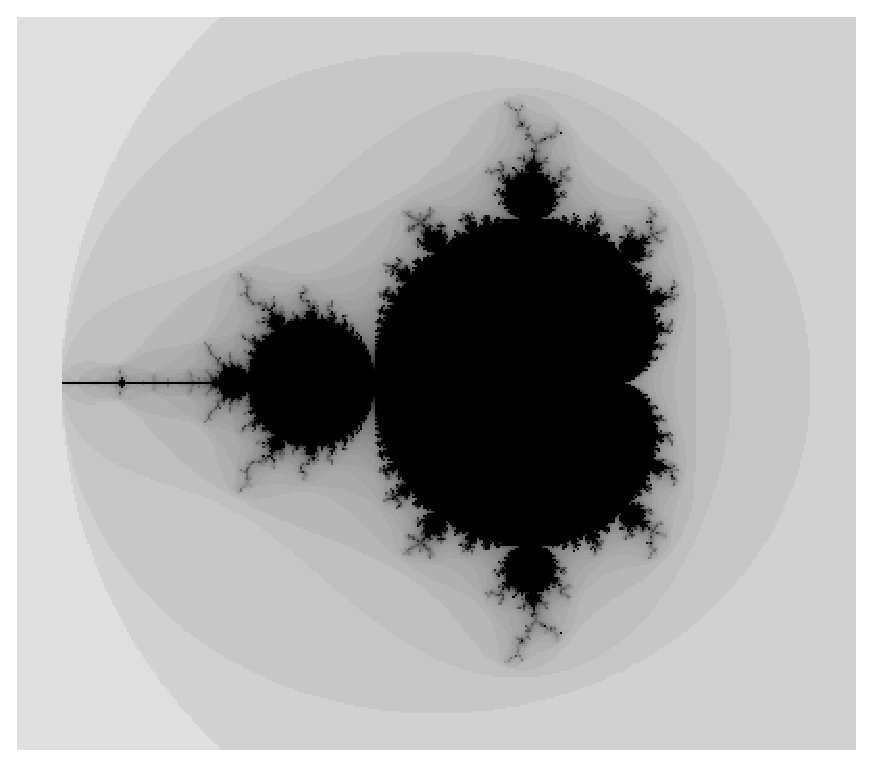
\includegraphics[height=0.35\textwidth]{figures/eud_mandel_64it} 
 & 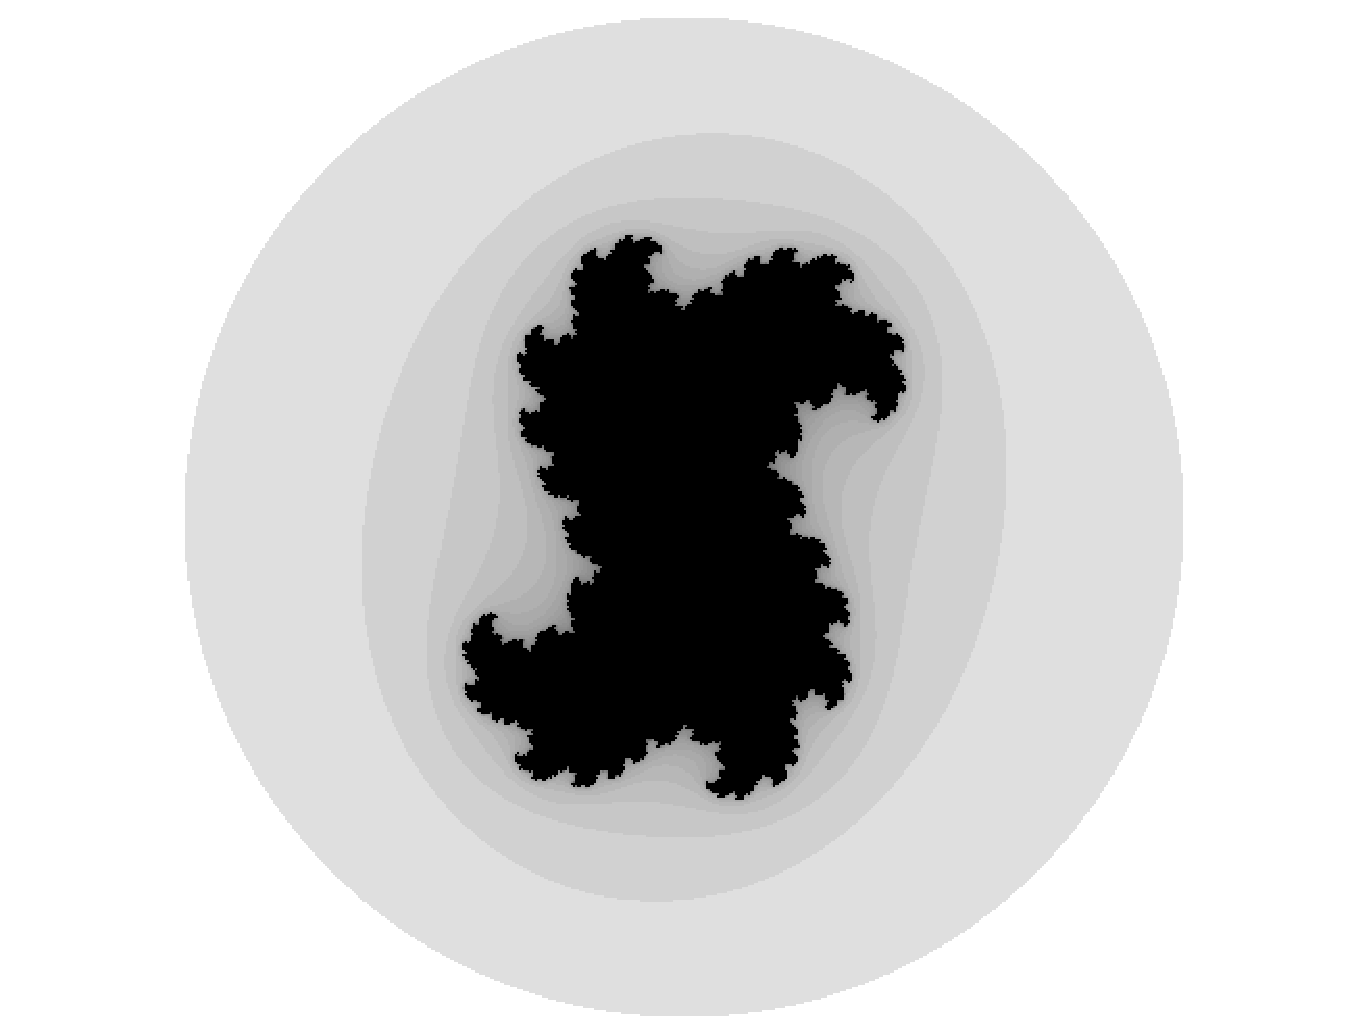
\includegraphics[height=0.35\textwidth]{figures/eud_julia_64it_0d35_0d203} \\
                          (a) & (b)
\end{tabular}
\caption{\label{fig:euclidean_sets}Two familiar plots: (a) The Mandelbrot set and
  (b) The Julia set associated with the constant $c = 0.35 + 0.203i$.}
\end{figure}

% FIXME: Awkward wording in this paragraph.

The classical Mandelbrot and Julia sets (figure \ref{fig:euclidean_sets}) are
probably the most famous images in recreational mathematics.  They are examples
of a form of fractal known as \emph{recurrence} or \emph{escape-time} fractals.
Each pixel in the image is associated with a point on the complex plane and
hence a complex number. A complex function is then repeatedly applied to this
number, the results of this iteration forming an \emph{orbit} for the original
point.  Should this orbit remain bounded, the original point is within the
fractal set.  If this orbit becomes unbounded, it is outside.

We assume a basic familiarity with the mechanism of generating Julia and
Mandelbrot sets along with the techniques used to calculate and plot them.
%We shall denote the Mandelbrot set as $\mathbb{M}$ and the
%Julia set associated with the complex number $c$ as $\mathbb{J}_c$.

% The same complex function generates both the Mandelbrot and Julia
% sets\cite{FRAC:Mandelbrot,FRAC:JuliaMandelBook}. It is worth noting that other
% functions could be used and hence many other escape-time fractals exist. Due to
% their similarity, there exist a number of theorems and conjectures which link
% the Mandelbrot and Julia sets in some way. For example, if $c \in \mathbb{M}$
% then the Julia set $\mathbb{J}_c$ is
% connected\cite{FRAC:JuliaAndMandelbrotSets}.  If $c$ is near the border of
% $\mathbb{M}$ then it is a Cantor set\cite{FRAC:JuliaAndMandelbrotSets}.

\section{Extending Complex Numbers}

In this section we present a simple Geometric Algebra based re-interpretation
of complex numbers\cite{anthonyChina} which reduces exactly to the usual complex algebra in the
2-d plane. We shall denote complex numbers in italics and embolden vectors to
distinguish them.

Existing extensions of complex numbers\cite{FRAC:HypercomplexIterations} have
been explicitly defined via co-ordinates specifying weighted sums of real and
multiple imaginary basis elements. We seek to form a co-ordinate free analog 
utilizing Geometric Algebra with the following goals: a) that, being
co-ordinate free and dimension agnostic, it will generalize easily to higher
dimensions and b) the co-ordinate free nature of the approach allows for
extensions to non-Euclidean geometries. In addition we wish to ground the
representation firmly in geometry without the creation of further `imaginary'
components in the hope that it will generate a greater geometric insight into
the famous Mandelbrot and Julia sets.

We firstly note that there is a `preferred direction' on the complex plane, the
real axis. We represent this direction via the unit vector ${\mathbf e}_r$
which points along this preferred direction in our target space. Just as
complex numbers can be represented as points on the complex plane, we represent
our `numbers' as vectors pointing to the location of points in space.

With this framework in place, we propose the following product as a good analog
of the complex product.

\begin{definition}[The complex geometric product]
The product ${\mathbf a} \complexprod {\mathbf b}$ is defined, for vectors 
${\mathbf a}, {\mathbf b}$ in terms of the geometric 
product\cite{hestenes,WarehamThesis} as
\begin{equation}
{\mathbf a} \complexprod {\mathbf b} \equiv {\mathbf a}{\mathbf e}_r{\mathbf b}.
\end{equation}
\end{definition}

Let us explore the properties of this product. We firstly restrict ourselves to
two-dimensions to show that the group generated via the complex geometric
product and $\mathbb{R}^2$ is isomorphic to the familiar group for complex
arithmetic.  Recalling that we have a preferred direction ${\mathbf e}_r$, we
may, in two-dimensions, find a direction orthogonal to ${\mathbf e}_r$
represented via the unit vector ${\mathbf e}_i$.  Any point in the plane may
now be resolved into components parallel to these basis directions:
\begin{equation}
{\mathbf z} = z_r{\mathbf e}_r + z_i{\mathbf e}_i.
\end{equation}

Consider the complex geometric product between two 2-d vectors, ${\mathbf a}$ 
and ${\mathbf b}$.
\begin{align*}
{\mathbf a} \complexprod {\mathbf b} & = {\mathbf a}{\mathbf e}_r{\mathbf b} \\
&= {\mathbf a}{\mathbf e}_r(b_r{\mathbf e}_r + b_i{\mathbf e}_i) \\
&= {\mathbf a}(b_r + b_i{\mathbf e}_r{\mathbf e}_i) \\
&= (a_r{\mathbf e}_r + a_i{\mathbf e}_i)(b_r + b_i{\mathbf e}_r{\mathbf e}_i) \\
&= (a_r b_r{\mathbf e}_r  + a_r b_i{\mathbf e}_i) +
   (a_i b_r{\mathbf e}_i - a_i b_i{\mathbf e}_r)\\
&= (a_r b_r - a_i b_i)\,{\mathbf e}_r  + (a_rb_i + a_ib_r){\mathbf e}_i.
\end{align*}
If one associates ${\mathbf e}_r$ with the real-axis and ${\mathbf e}_i$ with
the imaginary axis, one observes this to be equivalent to the usual complex
product.

We postulate that the complex geometric product may be generalized to higher
dimension by simply using higher-dimension vectors when calculating the product.
This postulate is justified by considering the action of the complex geometric
product on four dimensional vectors. By direct substitution it is easily verified
that it is isomorphic to the quaternion product used in
\cite{FRAC:HypercomplexIterations}.
Complex addition, which is essentially component-wise addition, reduces to 
vector addition within this framework.

\section{Higher Dimension Fractals}

In this section we extend the familiar two dimensional escape-time fractals to
higher dimension.  This turns out to be remarkably easy since the mapping is
co-ordinate free; we simply remove the constraint that the vectors representing
points on the set need be in $\mathbb{R}^2$.

We may now define generalized Mandelbrot and Julia sets based upon
a new vector recurrence relation.

\begin{definition}\label{def:gen_f(r)}
We define a vector analog of the complex function $f(z, c) = z^2 + c$ to be 
$f(\mathbf{x}, \mathbf{c})$ where
\begin{equation}
f(\mathbf{x}, \mathbf{c}) = \mathbf{x}\complexprod\mathbf{x} + \mathbf{c}
\end{equation}
and $f^{(n)}(\mathbf{x}, \mathbf{c})$ is the $n$-th application of 
$f(\cdot)$ to $\mathbf{x}$.
\end{definition}

\subsection{The Generalized Mandelbrot Set}

We can now reformulate the definition of the Mandelbrot set in a co-ordinate
free, dimension agnostic manner. 

\begin{definition}%[The generalized Mandelbrot set]
The generalized Mandelbrot set, $\mathbb{M}_k$, in $\mathbb{R}^k$ 
    is defined as
\begin{equation}
\mathbb{M}_k = 
\left\{\mathbf{c} \in \mathbb{R}^k 
: \lim_{n \rightarrow \infty} f^{(n)}(\mathbf{0}, \mathbf{c}) < \infty \right\}.
\end{equation}
\end{definition}

%We can now reformulate our definition of the Mandelbrot set in a co-ordinate
%free, dimension agnostic manner. 
This definition may be codified into the following algorithm which outlines the mechanism
for testing if the $n$-dimensional point $\mathbf{c}$ lies within the 
$n$-dimensional Mandelbrot set, $\mathbb{M}_n$.

\begin{enumerate}
\item $\mathbf{c} \leftarrow$ Location of point to test for inclusion in $\mathbb{M}_n$
\item $\mathbf{x} \leftarrow \mathbf{0}$
\item $k \leftarrow 0$ \emph{\{ Iteration counter \}}
\item $\mathbf{x} \leftarrow \mathbf{x} \complexprod \mathbf{x} + \mathbf{c}$ \label{loopstart1}
\item $k \leftarrow k + 1$
\item if $\mathbf{x}^2 > 4$ then
  \begin{enumerate}
  \item output $\mathbf{c} \notin \mathbb{M}_n$
  \item exit
  \end{enumerate}
\item if $n > $ maximum iteration count then
  \begin{enumerate}
  \item output $\mathbf{c} \in \mathbb{M}_n$
  \item exit
  \end{enumerate}
\item goto \ref{loopstart1}
\end{enumerate}

We terminate the algorithm when $\mathbf{x}^2 > 4$ since beyond that point,
the orbit will always tend to infinity.

One can then generate a plot of points within the set and colour those points
outside depending on the number of iterations that were performed before
the magnitude of $\mathbf{x}$ exceeded $2$.

\subsection{The Generalized Julia Set}

We may generalize the Julia set in an analogous manner.

\begin{definition}[The generalized Julia set]
The generalized Julia set, $\mathbb{J}_{\mathbf{c},k}$, in $\mathbb{R}^k$
which is associated with the vector $\mathbf{c} \in \mathbb{R}^k$ is given by
\begin{equation}
\mathbb{J}_{\mathbf{c},k} = 
\left\{\mathbf{x} \in \mathbb{R}^k
: \lim_{n \rightarrow \infty} f^{(n)}(\mathbf{x},\mathbf{c}) < \infty \right\}.
\end{equation}
\end{definition}

As an entertaining diversion---and in order to visualize this generalized 
Julia set---we extend the method in
\cite{FRAC:HypercomplexIterations} of ray-tracing quaternionic escape-time
fractals to the generalized Geometric Algebra fractals developed above.
Ray-tracing of fractals is achieved by finding some distance function
$d(\mathbf{x};\mathbf{c})$ which gives the minimum distance to $\mathbb{J}_{\mathbf{c},k}$
from the point $\mathbf{x}$. 

In \cite{FRAC:HypercomplexIterations} it was shown, for the complex number form
of the escape-time fractals above, that such a distance function, along a unitary
direction $u$, at
a point $z$ in the complex plane, $d(z,c,u)$ was bounded from below by
\begin{equation}
d(z,c,u) > \lim_{n \rightarrow \infty}\,\frac{|f^{(n)}(z,c)|}{2|f'^{(n)}(z,c)|}
\log|f^{(n)}(z,c)|
\end{equation}
where $f'^{(n)}(z,c)$ is the directional derivative of $f^{(n)}(z,c)$ along $u$:
\begin{eqnarray}
f'^{(n)}(z,c) &=& \nabla_u\;f^{(n)}(z,c)\\
&=& \nabla_u \left[ f^{(n-1)}(z,c)\;f^{(n-1)}(z,c) + c \right] \\
&=& 2uf^{(n-1)}(z,c)\ .
\end{eqnarray}
The complex values $z$ and $c$ are
dictated by the type of fractal as described above.

%The proof follows through exactly when the complex geometric product is
%substituted in and can be trivially extended to higher dimension.  
Further, each stage of the proof presented in
\cite{FRAC:HypercomplexIterations} may have the complex geometric product we
outlined above used instead of the usual complex product and in a way which
generalizes to higher dimension. Specifically
\begin{equation}
d(\mathbf{x}, \mathbf{c}, \mathbf{u}) > 
   \lim_{n \rightarrow \infty}\,\frac{|\mathbf{x}_n|}{2|\delta^{\mathbf{x}_{n}}_\mathbf{u}
f(\mathbf{x}_{n}, \mathbf{c})|}\log|\mathbf{x}_n|
\end{equation}
where $\mathbf{x}_n = f(\mathbf{x}_{n-1})$, $\mathbf{x}_0 = \mathbf{x}$ and the operator 
$\delta^\mathbf{x}_\mathbf{a}$ is the vector differential in the direction of
$\mathbf{a}$:
\begin{equation}
\delta^{\mathbf{x}}_\mathbf{a} f(\mathbf{x}, \mathbf{y}) =
\lim_{\epsilon \rightarrow 0} 
\frac{f(\mathbf{x} + \epsilon \mathbf{a}, \mathbf{y}) - f(\mathbf{x}, \mathbf{y})}
{\epsilon \magof{\mathbf{a}}}.
\end{equation}
It can easily be verified that
\begin{equation}
|\delta^{\mathbf{x}_{n}}_\mathbf{u} f(\mathbf{x}_{n}, \mathbf{c})|
 = |\mathbf{u} \complexprod \mathbf{x}_{n-1} + \mathbf{x}_{n-1} \complexprod \mathbf{u}|
 < 2 |\mathbf{u} \complexprod \mathbf{x}_{n-1}|
\end{equation}
and hence
\begin{equation}
d(\mathbf{x}, \mathbf{c}, \mathbf{u}) > 
   \lim_{n \rightarrow \infty}\,\frac{|\mathbf{x}_n|}{4|
   \mathbf{u} \complexprod \mathbf{x}_{n-1}
   |}\log|\mathbf{x}_n|\ .
   \label{eqn:dist-low-bound}
\end{equation}
% where $\mathbf{x}_n = f(\mathbf{x}_{n-1})$ and the operator 

Once a distance function (or a lower bound thereof) is available ray tracing
becomes possible. Rays of light are traced back from a point in the image
plane of an imaginary camera to the scene. For a particular ray the algorithm
to trace the fractal is as follows.

\begin{enumerate}
\item $\mathbf{u} \leftarrow$ a unit vector pointing along the ray direction
\item $\mathbf{x} \leftarrow $ camera origin
\item $\tau \leftarrow$ tolerance for deciding that a point is in the set
\item $d_- \leftarrow d(\mathbf{x}, \mathbf{c}, \mathbf{u})$ \label{loopstart2} $\quad$ \emph{\{ Compute lower bound via RHS of (\ref{eqn:dist-low-bound}). \}}
\item if $d_- < \tau$ then
  \begin{enumerate}
  \item output $\mathbf{x} \in \mathbb{J}_{\mathbf{c}}$
  \item exit
  \end{enumerate}
\item $\mathbf{x} \leftarrow \mathbf{x} + d_-\mathbf{u}$.
\item goto \ref{loopstart2}
\end{enumerate}

\begin{figure}
\centering
\includegraphics[width=\textwidth]{figures/generated-fractal-sm}
\caption{\label{fig:5djulia}An illustration of a ray-traced
three dimensional slice through a four dimensional Julia set.
}
\end{figure}

Once the intersection point is found the fractal must be correctly lit.
This involves calculating the surface normal. An approximation to the normal
can be found by modelling the fractal around the intersection as a plane
passing through neighbouring intersection points. The normal of this plane can
then be used for lighting. Figure \ref{fig:5djulia} shows a slice through a 5d
Julia set rendered with this technique.

\section{Moving to Hyperbolic Geometry}

So far all our fractals have been generated using the Euclidean geometry of
flat space. In this section we extend our algorithm using the non-Euclidean
tools given to us by \emph{Conformal Geometric
Algebra}\cite{wareham:iwmm,GA:llw,anthonyChina}. 

Hyperbolic geometry is usually represented in two dimensions on the
\emph{Poincar\'e disc}. This is a unit disc centred on the origin
onto which all space is mapped. A metric is defined within the
disc\cite{brannan}, along with a set of congruence transformations.
The boundary circle of the disc represents the points at infinity and everywhere
outside the disc is inaccessible to the hyperbolic geometry. Straight lines,
called $d$-lines\cite{brannan}, are represented by circular arcs which
erupt normal to the boundary circle. 

Perhaps one of the most famous examples of this geometry is given in Escher's
\emph{Circle Limit} series of wood prints, an example of which is recreated in
figure \ref{fig:circlelimit}. In these prints infinite tessellations of
hyperbolic space are represented via a mapping onto the Poincar\'e disc and
they show the circular nature of $d$-lines, although Escher was unaware of the
Poincar\'e disc model at the time the prints were made. This figure may
itself be used to demonstrate the non-commutativity of translation. In the
figure arrows are overlayed such that arrows of the same color are
parallel and the same length. Moving first along a green arrow then two
reds leads one to a different position than initially following the red 
arrows and \emph{then} the green.

\begin{figure}
\centering
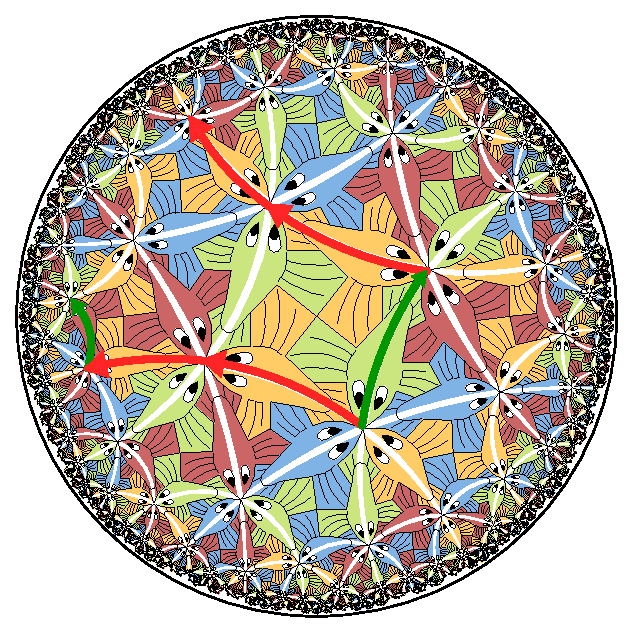
\includegraphics[width=0.9\textwidth]{circlimit-overlay} \\
\caption{\label{fig:circlelimit}
A re-creation of Escher's \emph{Circle Limit III}, 
a depiction of hyperbolic geometry on the Poincar\'e disc
taken from \cite{transhyp} with
an illustration of the non-commutativity of translation on the
hyperbolic grid overlayed.
}
\end{figure}

We procede by re-expressing
our complex geometric product in terms of the geometric operations it performs.
Viewed using an eye atuned to Geometric Algebra, our function $f(\mathbf{x},
\mathbf{c}) = \mathbf{x}\complexprod\mathbf{x} + \mathbf{c}$ performs three
operations.  Firstly the $\mathbf{x}\complexprod\mathbf{x}$ step reduces to a
reflection of a point on the preferred axis about $\mathbf{x}$ and a dilation
so that its distance from the origin becomes $\mathbf{x}^2$. The final step is
to translate the resulting point along $\mathbf{c}$.

The reflection step is equivalent to a rotation in the
$\mathbf{e}_r$-$\mathbf{x}$ plane so that the angle from $\mathbf{e}_r$ to
$\mathbf{x}$ is doubled.

We shall develop an analog of this step for the non-Euclidean hyperbolic
geometry of the Poincar\'e disc\cite{brannan}. 
To this end, we shall explicitly separate out
the geometric steps described above into elements of a Geometric algebra
termed \emph{rotors}\cite{wareham:amdo_rotor} which perform the
Euclidean rotation $r_e(\mathbf{x})$, the Euclidean dilation, $d_e(\mathbf{x})$
and the Euclidean translation,
$t_e(\mathbf{x}, \mathbf{c})$ giving us a Euclidean version of $f(\mathbf{x},
\mathbf{c})$ as
\begin{equation}
f_e(\mathbf{x}, \mathbf{c}) = t_e(d_e(r_e(\mathbf{x})), \mathbf{c})
\end{equation}
where
\begin{equation}
r_e(\mathbf{x}) = \frac{\mathbf{x}\complexprod\mathbf{x}}{\sqrt{\mathbf{x}^2}}, \qquad
d_e(\mathbf{x}) = \mathbf{x}^2 \frac{\mathbf{x}}{\sqrt{\mathbf{x}^2}}, 
\quad\hbox{and}\quad
t_e(\mathbf{x}, \mathbf{c}) = \mathbf{x} + \mathbf{c}.
\end{equation}

We now seek to form analagous functions $r_h(\cdot)$, $d_h(\cdot)$ and
$t_h(\cdot)$ for the hyperbolic geometry to allow us to form a
hyperbolic form of $f(\cdot)$, $f_h(\mathbf{x}, \mathbf{c})$.

We firstly note that rotation about the origin in the Poincar\'e disc is
identical to Euclidean rotation and so $r_h(\mathbf{x})
\equiv r_e(\mathbf{x})$. We shall consider dilation in due
course but for now we concentrate on the translation function $t_h(\cdot)$.

In the Conformal Model of Geometric Algebra\cite{WarehamThesis}, we construct
an element known as a \emph{translator} which acts multiplicitively upon
some representation of a point to give the representation of a translated
point.

In the case of Euclidean geometry, a point $\mathbf{x}$ is represented by
$F(\mathbf{x})$ where
\begin{equation}
F(\mathbf{x}) = \frac{\mathbf{x}^2}{2}n + \mathbf{x} - \frac{1}{2}\bar{n}
\end{equation}
and $n$, $\bar{n}$ are defined in \cite{WarehamThesis}. A translator,
$T_\mathbf{c}$, can then be formed such that
\begin{equation}
F(\mathbf{x} + \mathbf{c}) = T_\mathbf{c} F(\mathbf{x}) \tilde{T}_\mathbf{c}
\end{equation}
where $\tilde{T}_\mathbf{c}$ denotes the Geometric Algebra \emph{reversion} 
of $T_\mathbf{c}$. In the Euclidean case $T_\mathbf{c}$ is given
by
\begin{equation}
T_\mathbf{c} = 1 + \frac{n \mathbf{c}}{2}.
\end{equation}

In the Conformal Model, the translation of $\mathbf{x}$ along $\mathbf{c}$ is
denoted $\mathbf{x} \oplus \mathbf{c}$ and defined as
\begin{equation}
\mathbf{x} \oplus \mathbf{c} \equiv F^{-1}(T_\mathbf{c}
  F(\mathbf{x}) \tilde{T}_\mathbf{c}).
\end{equation}
Hence we may re-define our translation function as $t_e(\mathbf{x}, \mathbf{c})
= \mathbf{x} \oplus \mathbf{c}$.

Using the Euclidean definitions of $F(\mathbf{x})$ and $T_\mathbf{c}$ above
it can be shown by direct substitution that $\mathbf{x} \oplus \mathbf{c} \equiv
\mathbf{c} \oplus \mathbf{x}$.

The great power of the Conformal Model is that the work required to
move between geometries is only the work required to change the mapping function
$F(\cdot)$ and the definition of the translators. In \cite{WarehamThesis} the
corresponding mapping functions and translators for the Poincar\'e disc of
unit radius were shown to be
\begin{equation}
F_h(\mathbf{x}) = \frac{1}{1 - \mathbf{x}^2} (\mathbf{x}^2n + 2\mathbf{x} - \bar{n}),
\quad
T_{\mathbf{c},h} = \frac{1}{\sqrt{1 - \mathbf{x}^2}} (1 + \bar{e} \mathbf{x}).
\end{equation}
where $\bar{e}$ is defined in \cite{WarehamThesis}.
From these we can define the hyperbolic translation of $\mathbf{x}$ along
$\mathbf{c}$, $\mathbf{x} \oplus_h \mathbf{c}$. Interestingly, in general
$\mathbf{x} \oplus_h \mathbf{c} \ne \mathbf{c} \oplus_h \mathbf{x}$ and so we
shall, at the end of this process, obtain two different forms for the
Mandelbrot and Julia sets depending on the order in which we perform the
$\oplus_h$ operation. 

We now address the problem of handling dilations. The dilation function
takes a point $\mathbf{x}$ with distance from the origin $D_h(\mathbf{x})$ and
returns a point which is on the line joining the origin and $\mathbf{x}$
but has distance $D^2_h(\mathbf{x})$ from the origin. Pleasingly, lines from the
origin on the Poincar\'e disc are also straight Euclidean lines and so we
need only concern ourselves with getting the distance correct.

In \cite{WarehamThesis}, an appropriate distance function for the Poincar\'e
disc was stated to be
\begin{equation}
D_h(\mathbf{x}) = \mathrm{sinh}^{-1}\left(\sqrt{
\frac{\mathbf{x}^2}{1 - \mathbf{x}^2}
}\right)
\end{equation}
and hence, the Euclidean distance from the origin of a point with
hyperbolic distance $D_h(\mathbf{x})$, $D_e(D_h(\mathbf{x}))$ is
\begin{equation}
D_e(D_h(\mathbf{x})) = \frac{
\mathrm{sinh}(D_h(\mathbf{x}))
}{
\sqrt{1 + \mathrm{sinh}^2(D_h(\mathbf{x}))}
}.
\end{equation}

Our dilation function should therefore dilate the point so that its
hyperbolic distance from the origin is squared or, specifically,
\begin{equation}
d_h(\mathbf{x}) = D_e(D_h^2(\mathbf{x})) \frac{\mathbf{x}}{\sqrt{\mathbf{x}^2}}.
\end{equation}

\begin{figure}
\centering
\includegraphics[width=0.85\textwidth]%
{figures/hyp_mandel_128it_1alttrans_v2} \\
(a) \\ \vskip1em
\includegraphics[width=0.85\textwidth]%
{figures/hyp_mandel_128it_0alttrans_v2} \\
(b)
\caption{\label{fig:hyperbolic_mandelbrot}
Plot of the Mandelbrot set on the Poincar\'e disc using
a) $f_{h,1}(\mathbf{x}, \mathbf{c})$ and
b) $f_{h,2}(\mathbf{x}, \mathbf{c})$.
}
\end{figure}

\begin{figure}
\centering
\includegraphics[width=0.85\textwidth]%
{figures/hyp_julia_128it_1alttrans_0d35_0d203_v2} \\
(a) \\ \vskip1em
\includegraphics[width=0.85\textwidth]%
{figures/hyp_julia_128it_0alttrans_0d35_0d203_v2} \\
(b)
\caption{\label{fig:hyperbolic_julia}
Plot of a Julia set on the Poincar\'e disc using
(a) $f_{h,1}(\mathbf{x}, \mathbf{c})$ and
(b) $f_{h,2}(\mathbf{x}, \mathbf{c})$. In both cases
$\mathbf{c} = 0.35\mathbf{e}_1 + 0.203\mathbf{e}_2$.
}
\end{figure}

Putting these all together, we obtain two possible hyperbolic analogs for our
function $f(\mathbf{x}, \mathbf{c})$:
\begin{equation}
f_{h,1}(\mathbf{x}, \mathbf{c}) = d_h\left(
\frac{\mathbf{x}\complexprod\mathbf{x}}{\sqrt{\mathbf{x}^2}}
\right) \oplus_h \mathbf{c}
\end{equation}
\begin{equation}
f_{h,2}(\mathbf{x}, \mathbf{c}) = 
\mathbf{c} \oplus_h 
d_h\left(
\frac{\mathbf{x}\complexprod\mathbf{x}}{\sqrt{\mathbf{x}^2}}
\right).
\end{equation}

\subsection{The Hyperbolic Julia Set}

The two possible hyperbolic Mandelbrot sets are shown in figure
\ref{fig:hyperbolic_mandelbrot} and two particular hyperbolic Julia sets are
shown in figures \ref{fig:hyperbolic_julia}.  The two sub-figures show the sets
with the same parameters but differing methods of representing $x \mapsto x+c$.
It is interesting to note that not only are the fractals different but they
have different overall shape and behaviour. It is also worth remarking that,
geometrically, there is no preferred form of the translation representation and
so both these montages are equally valid images of hyperbolic Julia sets.  This
leads to the interesting conclusion that, whilst there is only one family of
Euclidean Julia sets, for non-commuting geometries there are two.

\section{Conclusions}

In this paper we have developed a co-ordinate free analog of complex arithmetic
and shown how the common escape-time fractals may be re-expressed using this
analog. This leads naturally to higher-dimension versions.

In addition to the straight-forward extension of escape-time fractals in
Euclidean geometries, we further extended our analog into the non-Euclidean geometry of the
Poincar\'e disc. The non-commuting nature of vector translation in this
geometry lead to two distinct forms of the Mandelbrot and associated
Julia sets within the disc.

\bibliography{header,fractals,fractal_coding,bibliography}

\end{document}

